\documentclass{beamer}
\usetheme{Singapore}
\usepackage{changepage}

%\usepackage{pstricks,pst-node,pst-tree}
\usepackage{amssymb,latexsym}
\usepackage{tikz}
\usepackage{graphicx}
\usepackage{fancyvrb}
\usepackage{hyperref}
\usepackage{fancybox}
\usepackage[listings]{tcolorbox}

\definecolor{codegreen}{rgb}{0,0.6,0}
\definecolor{codegray}{rgb}{0.5,0.5,0.5}
\definecolor{codepurple}{rgb}{0.58,0,0.82}
\definecolor{backcolour}{rgb}{0.95,0.95,0.92}

\lstdefinestyle{mystyle}{
    language=Python,
    backgroundcolor=\color{backcolour},   
    commentstyle=\color{codegreen},
    keywordstyle=\color{magenta},
    numberstyle=\tiny\color{codegray},
    stringstyle=\color{codepurple},
    basicstyle=\ttfamily\footnotesize,
    breakatwhitespace=false,         
    breaklines=true,                 
    captionpos=b,                    
    keepspaces=true,                 
    numbers=left,                    
    numbersep=5pt,                  
    showspaces=false,                
    showstringspaces=false,
    showtabs=false,                  
    tabsize=2,
    escapechar=|,
    frame=single
}

\lstset{style=mystyle}


\newcommand{\bi}{\begin{itemize}}
\newcommand{\li}{\item}
\newcommand{\ei}{\end{itemize}}
\newcommand{\Show}[1]{
\begin{center}
\shadowbox{\begin{minipage}{0.8\textwidth}
          #1
          \end{minipage}}
\end{center}
}
\newcommand{\arrow}{\ensuremath{\rightarrow}}

\newcommand{\uparr}{\ensuremath{\uparrow}}


\newcommand{\fig}[2]{\centerline{\includegraphics[width=#1\textwidth]{#2}}}

\newcommand{\bfr}[1]{\begin{frame}[fragile]\frametitle{{ #1 }}}
\newcommand{\efr}{\end{frame}}

\newcommand{\cola}{\begin{columns}\begin{column}{0.5\textwidth}}
\newcommand{\colb}{\end{column}\begin{column}{0.5\textwidth}}
\newcommand{\colc}{\end{column}\end{columns}}


\title{Think Python 2e, Chapter 15 Notes}
\author{Classes and Objects}

\begin{document}

\begin{frame}
\maketitle
\end{frame}

\bfr{A new data type: point}

To represent a two dimensional point in the plane, $(x,y)$, we could:
\bi
\li Use two variables, \lstinline{x} and \lstinline{y}
\li Use a list or tuple.
\li Use a dictionary with \lstinline{'x'} and \lstinline{'y'} as keys.
\li Create a new data type to represent points as objects.
\ei

\end{frame}
\bfr{A new data type}
\begin{lstlisting}
class Point:
    """Represents a point in 2-D space."""
\end{lstlisting}
\bi
\li
Defining a class named Point creates a {\bf class object}.
\li
The string is the documentation string,
or {\bf docstring}.
\li
Class names are traditionally capitalized.
\ei

\begin{lstlisting}
>>> Point
<class '__main__.Point'>
\end{lstlisting}
\bi
\li
Because Point is defined at the top level, 
its “full name” is \lstinline{__main__.Point}.
\ei
\end{frame}


\bfr{A new data type: {\tt Point}}
\begin{lstlisting}
class Point:
    """Represents a point in 2-D space."""
\end{lstlisting}
\bi
\li
The class object is like a factory for creating objects.
\li
 To create a Point, you call \lstinline{Point} as if it were a function.
 \ei
\begin{lstlisting}
>>> blank = Point()
>>> blank
<__main__.Point object at 0xb7e9d3ac>
\end{lstlisting}
\bi
\li
The return value is a reference to a \lstinline{Point}
 object.
\li
Creating a new object is called {\bf instantiation}.
\li The object is an {\bf instance} of the class.
\li The hex number is its location in memory.
\li In Python every object is an instance of some class.
\ei


\end{frame}

\bfr{Attributes}

User-defined objects can have {\bf attributes}.
\begin{lstlisting}
>>> blank.x = 3.0
>>> blank.y = 4.0
>>> '(%g, %g)' % (blank.x, blank.y)
'(3.0, 4.0)'
>>> distance = math.sqrt(blank.x**2 + blank.y**2)
>>> distance
5.0
\end{lstlisting}
State diagram:

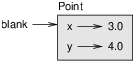
\includegraphics{statediagram15-01}

\end{frame}


\bfr{Functions of objects}


\begin{lstlisting}
def print_point(p):
    print('(%g, %g)' % (p.x, p.y))
\end{lstlisting}
\begin{lstlisting}
>>> print_point(blank)
(3.0, 4.0)
\end{lstlisting}

Objects are aliased, so if the function modifies
\lstinline{p}'s attributes, \lstinline{blank}'s attributes
 change, too.

\end{frame}

\bfr{A new data type: {\tt Rectangle}}

\begin{lstlisting}
class Rectangle:
    """Represents a rectangle. 

    attributes: width, height, corner.
    """
\end{lstlisting}

Are there other good representations?

What about tilted rectangles?

\end{frame}



\bfr{A new data type: {\tt Rectangle}}


\begin{lstlisting}
box = Rectangle()
box.width = 100.0
box.height = 200.0
box.corner = Point()
box.corner.x = 0.0
box.corner.y = 0.0
\end{lstlisting}

State diagram:
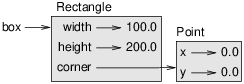
\includegraphics{statediagram15-02}

An object that is an attribute of
another object is {\bf embedded}.

\end{frame}

\bfr{Instances as return values}

\begin{lstlisting}
def find_center(rect):
    p = Point()
    p.x = rect.corner.x + rect.width/2
    p.y = rect.corner.y + rect.height/2
    return p
\end{lstlisting}
\begin{lstlisting}
>>> center = find_center(box)
>>> print_point(center)
(50, 100)
\end{lstlisting}

\end{frame}


\bfr{Objects are mutable}

\begin{lstlisting}
box.width = box.width + 50
box.height = box.height + 100
\end{lstlisting}
\begin{lstlisting}
def grow_rectangle(rect, dwidth, dheight):
    rect.width += dwidth
    rect.height += dheight
\end{lstlisting}
\begin{lstlisting}
>>> box.width, box.height
(150.0, 300.0)
>>> grow_rectangle(box, 50, 100)
>>> box.width, box.height
(200.0, 400.0)
\end{lstlisting}
\end{frame}

\bfr{Copying}
\bi
\li
Aliasing with objects can be problematic.
\li
The {\tt copy} module can copy anything.
\ei
\begin{lstlisting}
>>> p1 = Point()
>>> p1.x = 3.0
>>> p1.y = 4.0
>>> import copy
>>> p2 = copy.copy(p1)
>>> print_point(p1)
(3, 4)
>>> print_point(p2)
(3, 4)
>>> p1 is p2
False
>>> p1 == p2
False
\end{lstlisting}
\end{frame}

\bfr{Copying}

\begin{lstlisting}
>>> print_point(p1)
(3, 4)
>>> print_point(p2)
(3, 4)
>>> p1 is p2
False
>>> p1 == p2
False
\end{lstlisting}
\bi
\li
Python does not presume to know what counts as \lstinline{==}
\li
But you can tell it! (More on this later)
\ei
\end{frame}

\bfr{Shallow copy}
\begin{lstlisting}
>>> box2 = copy.copy(box)
>>> box2 is box
False
>>> box2.corner is box.corner
True
\end{lstlisting}

Object diagram:

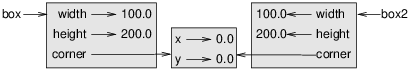
\includegraphics{statediagram15-03}
\end{frame}

\bfr{Deep copy}
\begin{lstlisting}
>>> box2 = copy.deepcopy(box)
>>> box2 is box
False
>>> box2.corner is box.corner
False
\end{lstlisting}

What does the object diagram look like?
\end{frame}

\bfr{Vocabulary}
\begin{description}
\li[class:]
A programmer-defined type. A class definition creates a new class object.
\li[class object:]
An object that contains information about a programmer-defined type. The class object can be used to create instances of the type.
\li[instance:]
An object that belongs to a class.
\li[instantiate:]
To create a new object.
\li[attribute:]
One of the named values associated with an object.
\li[embedded object:]
An object that is stored as an attribute of another object.
\end{description}
\end{frame}

\bfr{Vocabulary}
\begin{description}
\li[shallow copy:]
To copy the contents of an object, including any references to embedded objects; implemented by the copy function in the copy module.
\li[deep copy:]
To copy the contents of an object as well as any embedded objects, and any objects embedded in them, and so on; implemented by the deepcopy function in the copy module.
\li[object diagram:]
A diagram that shows objects, their attributes, and the values of the attributes.
\end{description}
\end{frame}


\end{document}
